\documentclass[prb,11pt,tightenlines,twocolumn,aps]{revtex4-1}
\usepackage{amsmath}    % need for subequations 
\usepackage{graphicx}   % need for figures 
\usepackage{verbatim}   % useful for program listings 
\usepackage{color}      % use if color is used in text 
\usepackage{subfigure}  % use for side-by-side figures 
\usepackage{hyperref}   % use for hypertext links, including those to external 
                        % documents and URLs 
%\usepackage{blindtext}  % fill text 
\usepackage[dvipsnames]{xcolor}
\usepackage{multirow}
%\usepackage[capitalize]{cleveref}
% \usepackage{showframe}
\usepackage[inline]{showlabels}
\input{/Users/reinaldo/Documents/tex_files/bmsdefinitions.tex}
% \input{/Users/bms/util/definitions}

\raggedbottom           % don't add extra vertical space

\begin{document}

\title{Pure Spin Current Injection in Hydrogenated Graphene Structures}
\author{Reinaldo Zapata-Pe\~na\textsuperscript{1},
        Bernardo S. Mendoza\textsuperscript{1},
        Anatoli I. Shkrebtii\textsuperscript{2}}
\affiliation{\textsuperscript{1}Centro de Investigaciones en \'Optica, Le\'on,
Guanajuato 37150, M\'exico}
\affiliation{\textsuperscript{2}University of Ontario, Institute of Technology,
Oshawa, ON, L1H 7L7, Canada}

\date{\today}

\begin{abstract}
perro
%\blindtext
\end{abstract}

\maketitle

%%%%%%%%%%%%%%%%%%%%%%%%%%%%%%%%%%%%%%%%%%%%%%%%%%%%%%%%%%%%%%%%%%%%%%%%%%%%%%
%%%%%%%%%%%%%%%%%%%%%%%%%%%%%%%%%%%%%%%%%%%%%%%%%%%%%%%%%%%%%%%%%%%%%%%%%%%%%%
%%%%%%%%%%%%%%%%%%%%%%%%%%                         %%%%%%%%%%%%%%%%%%%%%%%%%%%
%%%%%%%%%%%%%%%%%%%%%%%%%% I N T R O D U C T I O N %%%%%%%%%%%%%%%%%%%%%%%%%%%
%%%%%%%%%%%%%%%%%%%%%%%%%%                         %%%%%%%%%%%%%%%%%%%%%%%%%%%
%%%%%%%%%%%%%%%%%%%%%%%%%%%%%%%%%%%%%%%%%%%%%%%%%%%%%%%%%%%%%%%%%%%%%%%%%%%%%%
%%%%%%%%%%%%%%%%%%%%%%%%%%%%%%%%%%%%%%%%%%%%%%%%%%%%%%%%%%%%%%%%%%%%%%%%%%%%%%

\section{Introduction}
\label{sec:introduction}


\begin{figure}[ht!]
    \centering
    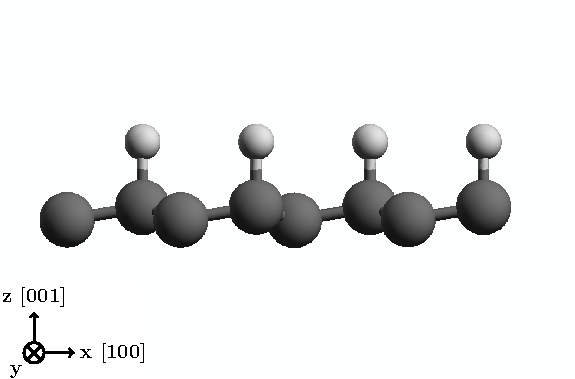
\includegraphics[width=\linewidth]{figures/upstruc2}
    \\
    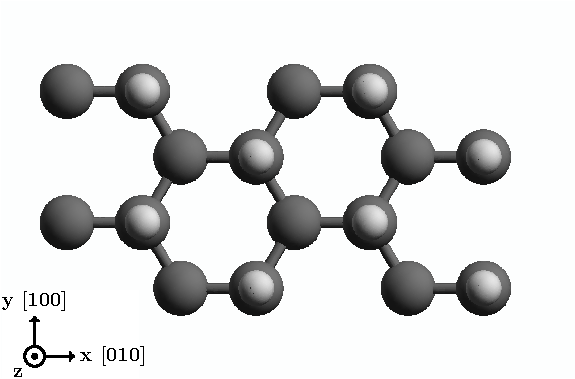
\includegraphics[width=\linewidth]{figures/upstruc1}
    \caption{Up structure}
    \label{fig:up-struc}
\end{figure}
\begin{figure}[ht!]
    \centering
    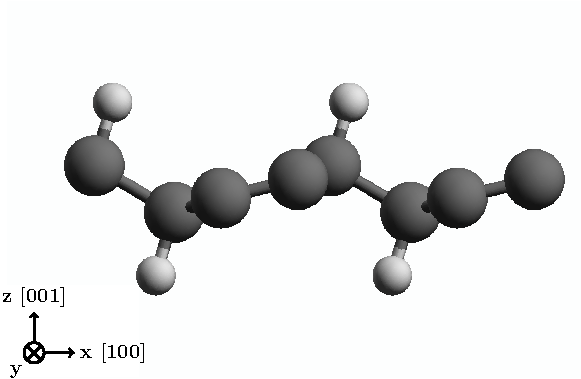
\includegraphics[width=\linewidth]{figures/altstruc2}
    \\
    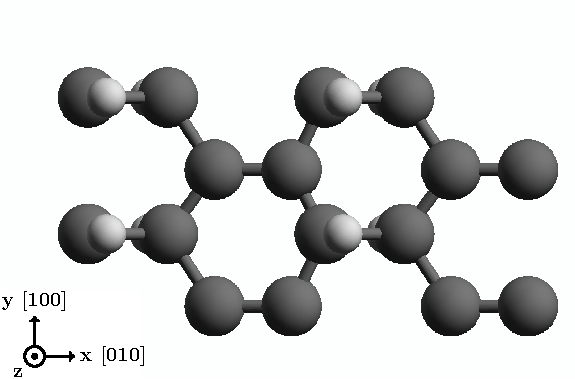
\includegraphics[width=\linewidth]{figures/altstruc1}
    \caption{Alt structure.}
    \label{fig:alt-struc}
\end{figure}


Spintronics is an emerging research field of electronics in which the
manipulation and transport of spin of electrons in a solid state 
media plays the determining role adding a new degree of freedom to the
conventional charge manipulation.\cite{wolfSC04,fabianAPS07}
% 
At present there is an increasing interest in attain the same level of control
over the transport of spin at micro or nano scales as has been done for the
flow of charge in typical electronic devices.\cite{awschalomNP2007} Some
semiconductor spintronics devices have been proposed \cite{majumdarAPL06,
dattaAPL90,gotteNat16,pershinPRB08} and some of them require spin polarized
electrical current \cite{awschalomSSBM13} or pure spin current (PSC).
% 
One of the difficulties to achieve the development of spin current and PSC
semiconductor devices is the fact that the spin relaxation time in a
semiconducting media is short disabling the spin transport and then resulting
in a no observable spin current.\cite{murakamiSc03}
% 
In PSCs there is no net
motion of charge; spin-up electrons move in a given direction while spin-down
electrons travel in the opposite one. This phenomena can result from spin
injection,\cite{malPRB03} Hall Effects,\cite{sinovaPRB04} interference of two
optical beams,\cite{bhatPRL00, najmaiePRB03} or one photon absorption of
linearly polarized light\cite{bhatPRL05} and has been observed in gallium
arsenide (GaAs),\cite{zhaoPRL2006, stevensPRL03} aluminum-gallium arsenide
(AlGaAs),\cite{stevensPRL03} and Co$_2$FeSi.\cite{kimuraNGPAM12}

Graphene, an allotrope of carbon with hexagonal 2D lattice structure presents
properties like fractional quantum Hall effect at room temperature, excellent
thermal transport properties, excellent conductivity\cite{heerscheNat07} and
strength \cite{geimNM07, reinaNL08, novoselov2S07, balandinNL08} being then a
perfect platform to be used in two-dimensions electronic systems; however most
electronic applications are disabled by the absence of a semiconducting gap.
Recent studies demonstrate that the band gap of graphene can be opened by
applying an electric field,\cite{zhangN09} reducing the surface
area,\cite{hanPRL07} or applying uniaxial strain.\cite{niACSN08} Another
possibility to open the gap is by doping; this has been successfully achieved
using nitrogen,\cite{weiNL2009} boron-nitrogen,\cite{guoIJ11}
silicon,\cite{colettiPRB10} noble-metals,\cite{varykhalovPRB10} and
hydrogen.\cite{eliasS09, guisingerNL09, samarakoonACSN10}
% 
Depending on the percentage of hydrogenation and spatial configurations of
hydrogen-carbon bonds, hydrogenated graphene can result in different spatial
configurations.
% 
In this paper we present two 50\% hydrogenated graphene noncentrosymmetric
structures both presenting a discernible band gap: the \emph{Up} structure,
shown in Fig. \ref{fig:up-struc}, has hydrogen atoms bonded to the carbon layer
only in the upper side of the structure while the \emph{Alt} structure, shown
in Fig. \ref{fig:alt-struc}, has hydrogen alternating in the upper and bottom
sides of the carbon slab.\cite{zapataPSB2016}

Using those structures we address a theoretical study of the spin velocity
injection (SVI) by one-photon absorption of linearly polarized light.
% 
% We calculated the responses for the particular cases when the spin of
% electrons is directed along the the $z$ Cartesian coordinate, perpendicular
% to the $xy$ plane of the structure, or for the case when the velocity is
% directed along the $x$ and $y$ Cartesian direction on the $xy$ plane of the
% structures.
{
% \color{red}
% 
Because we have 2D structures we made the analysis for tow cases. The first is
fixing the spin of the electrons along the $z$ Cartesian direction with the
velocity directed on the surface of the structure in the $xy$ plane. The second
is fixing the spin velocity in the $x$ or $y$ direction and the spin directed
in $xyz$.}
% 
The SVI is an optical effect that quantifies the velocity at which a PSC moves
along the Cartesian direction $\mathrm{a}$ with the spin of electron polarized
along the Cartesian direction $\mathrm{b}$. One photon absorption of linearly
polarized light can promote a distribution of electrons in $\mathbf{k}$ space
regardless the symmetry of the material resulting in a null electrical current.
Then, the electrons excited to the conduction bands at opposite $\mathbf{k}$
points will result in opposite spin polarizations producing no net spin
injection.\cite{bhatPRL05} If the crystalline structure of the material is
noncentrosymmetric the spin polarization injected at a given $\mathbf{k}$ point
could not vanish\cite{alvaradoPRL85, schmiedeskampPRL88} 
% 
{
% \color{red}
% 
and then, since the velocities of electrons at opposite $\mathbf{k}$ points are
opposite, a pure spin current will be produced. Since the structures presented
here are noncentrosymmetric, they are good candidates in which this effect can
be induced.}

This paper is organized as follows. In Section \ref{sec:theory} we present the
theory and formulas that describe PSC and SVI. In Section \ref{sec:results} we
describe the details of calculations and the corresponding SVI spectra for the
\emph{Up} and \emph{Alt} structures. Finally, we present our conclusions in
Section \ref{sec:conclusions}.


%%%%%%%%%%%%%%%%%%%%%%%%%%%%%%%%%%%%%%%%%%%%%%%%%%%%%%%%%%%%%%%%%%%%%%%%%%%%%%
%%%%%%%%%%%%%%%%%%%%%%%%%%%%%%%%%%%%%%%%%%%%%%%%%%%%%%%%%%%%%%%%%%%%%%%%%%%%%%
%%%%%%%%%%%%%%%%%%%%%%%%%%%%%%%%               %%%%%%%%%%%%%%%%%%%%%%%%%%%%%%%
%%%%%%%%%%%%%%%%%%%%%%%%%%%%%%%%  T H E O R Y  %%%%%%%%%%%%%%%%%%%%%%%%%%%%%%%
%%%%%%%%%%%%%%%%%%%%%%%%%%%%%%%%               %%%%%%%%%%%%%%%%%%%%%%%%%%%%%%%
%%%%%%%%%%%%%%%%%%%%%%%%%%%%%%%%%%%%%%%%%%%%%%%%%%%%%%%%%%%%%%%%%%%%%%%%%%%%%%
%%%%%%%%%%%%%%%%%%%%%%%%%%%%%%%%%%%%%%%%%%%%%%%%%%%%%%%%%%%%%%%%%%%%%%%%%%%%%%

\section{Theory} % (fold)
\label{sec:theory}


%%%%%%%%%%%%%%%%%%%%%%%%%%%%%%%%%%%%%%%%%%%%%%%%%%%%%%%%%%%%%%%%%%%%%%%%%%%%%%
%%%%%%%%%%%%%%%%%%%%%%%%%%% Theory: Spin velocity %%%%%%%%%%%%%%%%%%%%%%%%%%%%
%%%%%%%%%%%%%%%%%%%%%%%%%%%%%%%%%%%%%%%%%%%%%%%%%%%%%%%%%%%%%%%%%%%%%%%%%%%%%%


In this section, we report a summary of the theory that involves the PSC
phenomena from which rises the SVI treated in this paper.
 
{\color{red}
In PSCs there is no net motion of electrical charge and spin-up electrons move
in a given direction while spin-down electrons travel in the opposite one.
This effect can result from one photon absorption of linearly polarized light
by a semiconductor, with filled valence bands and empty conduction bands,
illuminated by light with photon energy larger than the energy gap.
% note 1
Using a single continuous linearly polarized laser beam, it is possible
to promote electrons in $\mathbf{k}$ space regardless the symmetry of the
system resulting in a net current equal to zero. 
% 
If the phenomena is produced in a noncentrosymmetric semiconducting media, the
electrons promoted to the conduction bands at opposite $\mathbf{k}$ points
can produce a net spin polarization different to zero\cite{alvaradoPRL85},
resulting in a PSC because the velocity of electrons
at opposite $\mathbf{k}$ points are in opposite directions.
}

%%%BMSD
The operator that describes the electronic PSC is written as
\begin{align}\label{z.1}
\hat K^{\rma\rmb}=\frac{1}{2}\left( \hat v^\rma \hat S^\rmb 
+\hat  S^\rmb \hat v^\rma\right) 
,
\end{align} 
where $\hat\bfv=[\hat\bfr,\hat H_0]/i\hbar$ is the velocity operator, with
$\hat \bfr$ the position operator,  $\hat H_0$ the unperturbed
ground state Hamiltonian, and
the Roman superscripts  indicate Cartesian coordinates. 
To obtain the expectation value of 
$\hat K^{\rma\rmb}$, we use the length gauge for the perturbing
Hamiltonian, written as
\begin{align}\label{z.2}
\hat H_{\text{p}}=-e\hat\bfr\cdot\bfE(t)
,
\end{align}   
where the electric field of the applied laser is given by
\begin{align}\label{z.3}
\bfE(t)= \bfE(\go)e^{-i\go t} + \bfE^*(\go)e^{i\go t}
.
\end{align}
In order to 
calculate the response of the system to $\bfE(t)$, one needs to
take into account the excited coherent superposition
of the spin-splited conduction bands inherent to the 
noncentrosymmetric 
semiconductors considered in this work.
%Although, this splitting is small [15,16], is required to obtain the
%correct results\cite{nastosPRB07}.
% The conduction bands in the 
% noncentrosymmetric  
% semiconductors  
% are spin split by a small amount,[15,16] typically
%   smaller than the energy width of the laser pulse, and so the pulse
%   excites a coherent superposition of the two conduction bands. Even
%   for very long pulses with narrow energy widths, dephasing effects
%   lead to an energy width of the bands large enough that spin-split
%   states can become quasidegenerate. 
To include the coherences, we follow Ref.~\onlinecite{nastosPRB05} and
use a multiple
scale approach that solves the equation of motion for the single
particle density matrix $\gr_{mn}(\bfk;t)$, leading to
\begin{align}\label{z.4}
&\frac{\partial \rho_{cc'}(\bfk)}{\partial t} =
\frac{e^{2}E^{\mathrm{a}}(\omega)E^{\mathrm{b*}}(\omega)}
{i \hbar^{2}}
\sum_{v}r^{\mathrm{a}}_{cv}(\bfk) r^{\mathrm{b}}_{vc'}(\bfk)
\nonumber\\
&\times 
\left( \frac{1}{\omega - \omega_{c'v}(\bfk) - i \epsilon} 
- 
\frac{1}{\omega - \omega_{cv}(\bfk) + i \epsilon} \right)
,
\end{align}
where we assumed that the conduction bands $c$ and $c'$
are quasidegenerate  states and we take $\ge\to 0$ at the end of the
calculation.  The spin-splitting of the valence ($v$) bands is very
small, and is neglected throughout this work.\cite{??} 
% 􏱈 are close to  
% one another, and that the pulse is short enough so that the energy
% width overlaps the two bands, the equation of motion can be
% solved. Leaving the details of the derivation to Ap- 
% pendix A, the result for the off-diagonal component 􏰠 􏱈, c  
%%%BMSU 
The matriz elements of any operator $\calo$ are given by
$\calo_{nm}(\bfk)=\bra{n\bfk}\hat\calo\ket{m\bfk}$,
where 
$H_{0}|n\mathbf{k}\rangle = \hbar \omega_{n}(\mathbf{k})|n\mathbf{k}\rangle$ 
with $\hbar \omega_{n}(\mathbf{k})$ the energy of the
electronic band $n$ at point $\mathbf{k}$ in the irreducible Brillouin zone
(IBZ),  $|n\mathbf{k}\rangle$ is the Bloch state, and 
$\go_{nm}(\bfk)=\go_{n}(\bfk)-\go_{m}(\bfk)$.
Using 
$\mathcal{O} = \mathrm{Tr}(\hat{\rho}\hat{\mathcal{O}})$
for the expectation value of an observable $\mathcal{O}$, 
where $\mathrm{Tr}$ denotes the trace, we obtain
\begin{align}\label{z.5}
\mathcal{O} 
%=&
%\int \frac{d^{3}k}{8\pi^{3}}\sum_{c} \langle c \mathbf{k} 
%| \hat{\rho} \hat{\mathcal{O}} |
%c\mathbf{k} \rangle \nonumber \\
=& 
\int \frac{d^{3}k}{8\pi^{3}} \sum_{cc'} \rho_{cc'}(\mathbf{k}) 
\mathcal{O}_{c'c}(\mathbf{k}),
\end{align}
where we used 
the closure
relationship $\sum_{n}|n\mathbf{k}\rangle \langle n\mathbf{k}| = 1$,
where $n=v,c$,
and the fact that $\rho_{vn}(\bfk)=\rho_{nv}(\bfk)=0$ for $n=c,c'$. 
Therefore, 
using  Eqs. \eqref{z.4} and \eqref{z.5},
the
rate of change of $\mathcal{O}$,
$\dot{\mathcal{O}} 
=
\mathrm{Tr} \left( \frac{\partial \hat{{\rho}}}{\partial t} \hat\calo \right)
$,
 is given by
\begin{align}
\dot{\mathcal{O}} 
&=\frac{e^{2}}{i\hbar^{2}} \int \frac{d^{3}k}{8\pi^{3}} 
\sum'_{cc'} \mathcal{O}_{c'c}(\bfk) 
r^{\mathrm{a}}_{cv}(\bfk)  r^{\mathrm{b}}_{vc'}(\bfk)  \times
\nonumber \\
& \left( \frac{1}{\omega - \omega_{c'v}(\bfk)  - i\epsilon} - 
\frac{1}{\omega - \omega_{cv}(\bfk)  + i\epsilon} \right)
E^{\mathrm{a}}(\omega) E^{\mathrm{b*}}(\omega)
\label{eq:dotO}
.
\end{align}
Replacing  $\hat\calo \rightarrow \hat{K}^{\mathrm{ab}}$, in 
above expression, one can show that
\begin{equation}
\dot{K}^{\mathrm{ab}}(\omega) =
\mu^{\mathrm{abcd}}(\omega)
E^{\mathrm{c}}(\omega) E^{\mathrm{d*}}(\omega),
\label{eq:dotk}
\end{equation}
where repeated cartesian are summed, and 
\begin{equation}\label{eq:mu}
\begin{aligned}
\mu^{\mathrm{abcd}}  (\omega) &
=
\frac{\pi e^{2}}{\hbar^{2}} \int 
\frac{d^{3}k}{8 \pi^{3}} \sum'_{vcc'}
  \delta(\omega-\omega_{cv}(\bfk) 
\\
\times\mathrm{Re} & \left[ K^{\mathrm{ab}}_{cc'}(\bfk) 
\left(  
r^{\mathrm{c}}_{vc'}(\bfk)   
r^{\mathrm{d}}_{cv }(\bfk)  +
(c \leftrightarrow d)  
\right) 
\right]
,  
\end{aligned}
\end{equation} 
is the pseudotensor that describes the rate of change of the  PSC process in semiconductors.
To derive above we used  
$
K^{\mathrm{ab}}_{nm}(\mathbf{-k}) = K^{\mathrm{ab*}}_{nm}(\mathbf{k}). 
$
that follows from time-reversal invariance. 
The prime $'$ in the sum means that $c$ and $c'$ are quasi degenerate states and the
sum only covers these states.  Since $\mu^{\mathrm{abcd}}(\omega)$ is real we
have that $\mu^{\mathrm{abcd}}(\omega) =
\mu^{\mathrm{abdc}}(\omega)$. 
We remark that Eq.~\eqref{eq:mu} 
 is the same as Eq. (3) of Bhat et al.\cite{bhatPRL05}
obtained by using the semiconductor optical Bloch equations.
Using the closure relation,
\begin{equation}
K^{\mathrm{ab}}_{cc'}(\mathbf{k}) = \frac{1}{2}
\sum_{l=v,c}
\left(v^{\mathrm{a}}_{cl}(\mathbf{k})S^{\mathrm{b}}_{lc'}(\mathbf{k})
+S^{\mathrm{b}}_{cl}(\mathbf{k}) v^{\mathrm{a}}_{lc'}(\mathbf{k})
\right)
.
\label{eq:velspimatelem}
\end{equation}

%%%%%%%%%%%%%%%%%%%%%%%%%%%%%%%%%%%%%%%%%%%%%%%%%%%%%%%%%%%%%%%%%%%%%%%%%%%%%%
%%%%%%%%%%%%%%%%%%%%%%%%%%%%%%%%%%%%%%%%%%%%%%%%%%%%%%%%%%%%%%%%%%%%%%%%%%%%%%

%\subsection{Spin velocity injection} % (fold)
%\label{sec:theory-pure_spin_current}
Now, we define the spin velocity injection (SVI) as
\begin{equation}\label{eq:vab-w}
\mathcal{V}^{\mathrm{ab}}(\omega) \equiv
\frac{\dot{K}^{\mathrm{ab}}(\omega)}{(\hbar/2) \dot{n}(\omega)},
\end{equation}  
that gives 
the velocity, along the direction $\mathrm{a}$, at which the spin moves polarized along the 
direction $\mathrm{b}$.
The carrier injection rate $\dot n(\go)$ is written as,\cite{nastosPRB05}
\begin{equation}
\dot{n}(\omega) =
\xi^{\mathrm{ab}}(\omega) E^{c }(\omega) E^{d*}(\omega),
\label{eq:dotn}
\end{equation}
where the tensor 
\begin{equation}\label{eq:xi}
\begin{aligned}
\xi^{\mathrm{ab}}(\omega)
&
=
\frac{2\pi e^{2}}{\hbar^{2}} \int 
\frac{d^{3}k}{8 \pi^{3}}
\\\nonumber
&\times \sum_{vc}
r^{\mathrm{a}}_{vc'}(\bfk)  
r^{\mathrm{b}}_{cv }(\bfk)  
\delta(\omega-\omega_{cv}(\bfk) 
, 
\end{aligned}
\end{equation}
is related to the imaginary part of the linear optical 
response tensor by
$\mathrm{Im}[\ge^{\rma\rmb}(\go)]=2\pi\ge_0\hbar\xi^{\rma\rmb}(\go)$.

The function $\calv^{\rma\rmb}(\go)$ allow us to quantify two very
important aspects of PSC. On one hand, we can fix the spin direction
along $\mathrm{b}$,   
and calculate the resulting electron velocity.  
On the other hand, we can fix de velocity of the electron
along $\mathrm{b}$,  and study the resulting direction along which the
spin is polarized.
To this end, the added advantage of  2D structures, besides choosing
them noncentrosymmetric, is that we can use an incoming linearly
polarized beam of light
at normal incidence, and use the  direction of the polarized  electric
field to control $\calv^{\rma\rmb}(\go)$.
Indeed, writing 
$\bfE(\omega) = E_0(\omega)(\cos\ga\,\hat\bfx+\sin\ga\,\hat\bfy)$
where $\alpha$ is the polarization angle, we obtain from
 Eq. \eqref{eq:vab-w}
that
\begin{widetext}
\begin{align}
\mathcal{V}^{\mathrm{ab}}(\omega,\alpha)
&= 
\frac{2}{\hbar\xi(\go)}
\left(\mu^{\mathrm{abxx}}(\omega)\cos^{2}\alpha + 
\mu^{\mathrm{abyy}}(\omega)\sin^{2}\alpha + 
\mu^{\mathrm{abxy}}(\omega)\sin 2\alpha\right)
\label{eq:vab-aw}
\end{align}
\end{widetext}
as for the structures chosen in this article,
$\xi^{\mathrm{xx}}(\go)=\xi^{\mathrm{yy}}(\go)\equiv\xi(\go)$, and $\xi^{\mathrm{xy}}(\go)=0$.
Now, we formalize our two options for $\calv^{\rma\rmb}$.
% 

% Two interesting possibilities to analyze the SVI are fixing the spin along $z$,
% directed perpendicularly to the surface of the structure, or fixing the
% velocity along $x$ or $y$ on the $xy$ plane of the structures. Also we can
% analyze the SVI contribution coming from each layer of the structure. In
% following subsections we present these three cases.

%%%%%%%%%%%%%%%%%%%%%%%%%%%%%%%%%%%%%%%%%%%%%%%%%%%%%%%%%%%%%%%%%%%%%%%%%%%%%%
%%%%%%%%%%%%%%%%%%%%%%%%%%%% Theory: Fixing spin %%%%%%%%%%%%%%%%%%%%%%%%%%%%%
%%%%%%%%%%%%%%%%%%%%%%%%%%%%%%%%%%%%%%%%%%%%%%%%%%%%%%%%%%%%%%%%%%%%%%%%%%%%%%

\subsection{Fixing spin}\label{sec:theory-fixspin}

Analyzing the SVI, Eq. \eqref{eq:vab-aw}, we define the magnitude of
the electron's in plane
velocity with it's spin polarized along the $\mathrm{b}$ direction as
\begin{equation}
\mathcal{V}_{\sigma^{\mathrm{b}}}(\omega,\alpha)
\equiv
\sqrt{
[\mathcal{V}^{\mathrm{xb}}(\omega,\alpha)]^{2}\ +
[\mathcal{V}^{\mathrm{yb}}(\omega,\alpha)]^{2}\ 
}, 
\label{eq:vs-mag}
\end{equation}
and define the angle at which the velocity is directed on the $xy$ plane as
\begin{equation}
\gamma_{\gs^\mathrm{b}} (\omega,\alpha)
=
\tan^{-1} \left( \frac{\mathcal{V}^{\mathrm{yb}}(\omega,\alpha)}
{\mathcal{V}^{\mathrm{xb}}(\omega,\alpha)} \right)
.
\label{eq:gamma-ang}
\end{equation}
% where this angle is measured in the counter-clockwise direction from the
% positive $x$. 
We also define two special angles
\begin{equation}
\gamma_{\gs^\mathrm{b}}^\parallel(\omega,\alpha) = \alpha, 
\label{eq:gamma-par} 
\end{equation}
and
\begin{equation}
\gamma_{\gs\mathrm{b}}^\perp(\omega,\alpha) = \alpha \pm 90^{\circ},
\label{eq:gamma-perp}
\end{equation}
corresponding to the electron velocity being parallel or perpendicular
the incoming polarization, 
respectively. The subscript $\gs^\rmb$ denotes the spin along $\rmb$.

%%%%%%%%%%%%%%%%%%%%%%%%%%%%%%%%%%%%%%%%%%%%%%%%%%%%%%%%%%%%%%%%%%%%%%%%%%%%%%
%%%%%%%%%%%%%%%%%%%%%%%%%%%% Theory: Fixing vel %%%%%%%%%%%%%%%%%%%%%%%%%%%%%%
%%%%%%%%%%%%%%%%%%%%%%%%%%%%%%%%%%%%%%%%%%%%%%%%%%%%%%%%%%%%%%%%%%%%%%%%%%%%%%


\subsection{Fixing velocity.}\label{sec:theory-fixvel}

Fixing the calculated velocity along $\rma=x$ or $\rma=y$
 we define it's corresponding magnitude as
\begin{align}
\mathcal{V}_{\mathrm{a}}&(\omega,\alpha) \equiv \nonumber \\
&\sqrt { 
[\mathcal{V}^{\mathrm{ax}}(\omega,\alpha)]^{2} +
[\mathcal{V}^{\mathrm{ay}}(\omega,\alpha)]^{2} +
[\mathcal{V}^{\mathrm{az}}(\omega,\alpha)]^{2} 
},
\label{eq:vv-mag}
\end{align}
from where we see that the spin would be oriented
in the $xyz$ system's coordinates
according to a polar angle
\begin{align}
\theta_{\mathrm{a}}  (\omega,\alpha)
=& 
\cos^{-1} \left( \frac{\mathcal{V}^{\mathrm{az}}(\omega,\alpha)}
{\mathcal{V}_{\mathrm{a}}(\omega,\alpha)} \right),
& 0 \leq &\theta \leq \pi, 
\label{eq:polar-ang}
\end{align}
and an azimuthal angle
\begin{align}
\varphi_{\mathrm{a}} (\omega,\alpha)
=& 
\tan^{-1} \left( \frac{\mathcal{V}^{\mathrm{ay}}(\omega,\alpha)}
{\mathcal{V}^{\mathrm{ax}}(\omega,\alpha)} \right),
& 0 \leq &\varphi \leq 2\pi.
\label{eq:azimuthal-ang} 
\end{align} 


%%%%%%%%%%%%%%%%%%%%%%%%%%%%%%%%%%%%%%%%%%%%%%%%%%%%%%%%%%%%%%%%%%%%%%%%%%%%%%
%%%%%%%%%%%%%%%%%%%%%%%%%%%%%%%%%%%%%%%%%%%%%%%%%%%%%%%%%%%%%%%%%%%%%%%%%%%%%%
%%%%%%%%%%%%%%%%%%%%%%%%%%%%%                   %%%%%%%%%%%%%%%%%%%%%%%%%%%%%%
%%%%%%%%%%%%%%%%%%%%%%%%%%%%%   R E S U L T S   %%%%%%%%%%%%%%%%%%%%%%%%%%%%%%
%%%%%%%%%%%%%%%%%%%%%%%%%%%%%                   %%%%%%%%%%%%%%%%%%%%%%%%%%%%%%
%%%%%%%%%%%%%%%%%%%%%%%%%%%%%%%%%%%%%%%%%%%%%%%%%%%%%%%%%%%%%%%%%%%%%%%%%%%%%%
%%%%%%%%%%%%%%%%%%%%%%%%%%%%%%%%%%%%%%%%%%%%%%%%%%%%%%%%%%%%%%%%%%%%%%%%%%%%%%

\section{Results} % (fold)
\label{sec:results}

\begin{table}[t]
\center
\begin{tabular}{ccccc}\\
\hline
\quad Layer \quad & \quad Atom \qquad & \multicolumn{3}{c}{Position [\AA]} \\
\cline{3-5}
\quad No.   \quad & \quad type \qquad & $x$ & $y$ & $z$  \\
\hline
1 & H & -0.61516 & -1.77416 &  0.73196 \\
1 & H &  0.61518 &  0.35514 &  0.73175 \\
2 & C & -0.61516 & -1.77264 & -0.49138 \\
2 & C & -0.61516 & -0.35600 & -0.72316 \\
2 & C &  0.61516 &  0.35763 & -0.49087 \\
\hline
\end{tabular}

\caption{Unit cell of \emph{Up} structure. Layer division, atom types and
positions for the \emph{Up} structure. The structure unit cell was divided in
two layers corresponding to hydrogen and carbon atoms.The corresponding layer
atom position is depicted in Fig. \ref{fig:up-struc} with the corresponding
number of layer.}
\label{tab:up-unitcell}
\end{table}
% 
% 
\begin{table}[t]
\center
\begin{tabular}{ccccc}\\
\hline
\quad Layer \quad & \quad Atom \qquad & \multicolumn{3}{c}{Position [\AA]} \\
\cline{3-5}
\quad No.   \quad & \quad type \qquad & $x$ & $y$ & $z$  \\
\hline
1 & H &  -0.61516 &  -1.42140 & \ 1.47237 \\
2 & C &  -0.61516 &  -1.73300 & \ 0.39631 \\
3 & C & \ 0.61516 & \ 1.73300 & \ 0.15807 \\
4 & C & \ 0.61516 & \ 0.42201 &  -0.15814 \\
5 & C &  -0.61516 &  -0.37396 &  -0.39632 \\
6 & H &  -0.61516 &  -0.68566 &  -1.47237 \\
\hline
\end{tabular}

\caption{Unit cell of \emph{Alt} structure. Layer division, atom types and
positions for the \emph{Alt} structure. The structure unit cell was divided in
six layers corresponding each one to atoms in different $z$ positions. The
corresponding layer atom position is depicted in Fig. \ref{fig:alt-struc} with
the corresponding number of layer.}
\label{tab:alt-unitcell}
\end{table}

We preset the results for 
and
$\mathcal{V}_{\sigma^{\mathrm{b}}}(\omega,\alpha)$ 
and
$\mathcal{V}_{\mathrm{a}}(\omega,\alpha)$ 
for the
C$_{16}$H$_{8}$-up  and C$_{16}$H$_{8}$-alt 
structures being both
noncentrosymmetric semi-infinite 2D carbon systems with 50\% hydrogenation in
different arrangements. We recall that the \emph{Up} structure has hydrogen
atoms only on the upper side of the carbon sheet while the \emph{Alt} structure
has alternating hydrogen atoms on the upper and bottom sides. Also we take the
hexagonal carbon lattice to be on the $xy$ plane for both structures, and the
carbon-hydrogen bonds on the perpendicular $xz$ plane, as depicted in Figs.
\ref{fig:up-struc} and \ref{fig:alt-struc}. The coordinates for the
\emph{Up} and \emph{Alt} unit cells of the structures are presented in Tables
\ref{tab:up-unitcell} and \ref{tab:alt-unitcell}. 

We calculated the self-consistent ground state and the Kohn-Sham
states using density functional theory in the local density approximation (DFT-
LDA) with a planewave basis using the ABINIT code \cite{gonzeCPC09}.
% 
We used Hartwigsen-Goedecker-Hutter (HGH) relativistic separable dual-space
Gaussian pseudopotentials \cite{hartwigsenPRB98} including the spin-orbit
interaction needed to calculate $\mu^{\mathrm{abcd}}(\omega,\alpha)$ presented
in Eq. \eqref{eq:mu}.
% 
The convergence parameters for the calculations of our results corresponding to
the \emph{Up} and \emph{Alt} structures are cutoff energies of 40\,Ha and
65\,Ha, resulting in LDA energy band gaps of 0.084\,eV and 0.718\,eV,
respectively. The energy eigenvalues and matrix elements for the \emph{Up} and
\emph{Alt} structures were calculated using 12802 $\mathbf{k}$ points and 14452
$\mathbf{k}$ points in the IBZ to integrate $\mu^{\mathrm{abcd}}(\go)$ and
$\xi^{\rma\rmb}(\go)$ using the linearized analytic tetrahedron method
(LATM).\cite{nastosPRB07} We neglect the anomalous velocity term
$\hbar(\bfgs\times\nabla V)/4m^2c^2$, where $V$ is the crystal potential, in
$\hat\bfv$ of Eq.~\eqref{z.1}, as this term is known to give small contribution
to PSC.\cite{bhatPRL05} Therefore, $[\hat\bfv,\hat\bfS]=0$ and Eq.~\eqref{z.1}
reduces to $\hat K^{\rma\rmb}=\hat v^\rma \hat S^\rmb=\hat S^\rmb \hat v^\rma$.


% 
% It is known that the DFT with LDA approximation misestimates the energy band
% gap of semiconductors. To correct this one has to include the many-body
% interaction using i.e. the so-called GW approximation but this technique has a
% very high computational cost and is out of the scope in this paper.
% Nevertheless, DFT still remains a mainstream tool for calculating diverse
% properties derived from the electronic band structure.

%%%%%%%%%%%%%%%%%%%%%%%%%%%%%%%%%%%%%%%%%%%%%%%%%%%%%%%%%%%%%%%%%%%%%%%%%%%%%%
%%%%%%%%%%%%%%%%%%%%%%%%%%% Results: Spin velocity %%%%%%%%%%%%%%%%%%%%%%%%%%%
%%%%%%%%%%%%%%%%%%%%%%%%%%%%%%%%%%%%%%%%%%%%%%%%%%%%%%%%%%%%%%%%%%%%%%%%%%%%%%

\subsection{SVI: Spin velocity injection} % (fold)
\label{sec:res-spin_velocity}

\begin{table}[b]
\begin{tabular}{cccccc}
\hline
\multirow{2}{*}{Structure \quad} & 
Kind of \quad & 
Pol. &
Energy & 
\multicolumn{2}{c}{$\mathcal{V}^{\mathrm{ab}}(\omega,\alpha)$}\\
\cline{5-6}
& system & Ang. & [eV] & $\mathrm{ab}$ \quad & [Km/s]\\
\hline
\emph{Up}    & 2D   & 35    & 0.084  & $\mathrm{yz}$ &  684.2    \\
             &      &       & 1.954  & $\mathrm{yz}$ &  293.9    \\
             &      &       & 1.958  & $\mathrm{yz}$ & -273.0    \\
\emph{Alt}   & 2D   & 150   & 0.720  & $\mathrm{yz}$ & -722.2    \\
             &      &       & 0.911  & $\mathrm{yz}$ & -357.8    \\
 CdSe        & bulk & 90    & 0.912  & $\mathrm{zz}$ &  -32.3    \\
 GaAs        & bulk & 90    & 2.326  & $\mathrm{xx}$ &  -29.9    \\
\hline
\end{tabular}

\caption{Comparison of the reported maxima values of
$\mathcal{V}^{\mathrm{ab}}$ for the different structures and their
corresponding polarization angle $\alpha$ and energy values of the incoming
beam at which the maxima is obtained.}
\label{tab:vab-str-comp}
\end{table}

%%%%%%%%%%%%%%%%%%%%%%%%%%%%%%%%%%%%%%%%%%%%%%%%%%%%%%%%%%%%%%%%%%%%%%%%%%%%%%
%%%%%%%%%%%%%%%%%%%%%%%%%% Res: mu & V^{ab} comparison %%%%%%%%%%%%%%%%%%%%%%%
\begin{figure}[t]
    \centering
    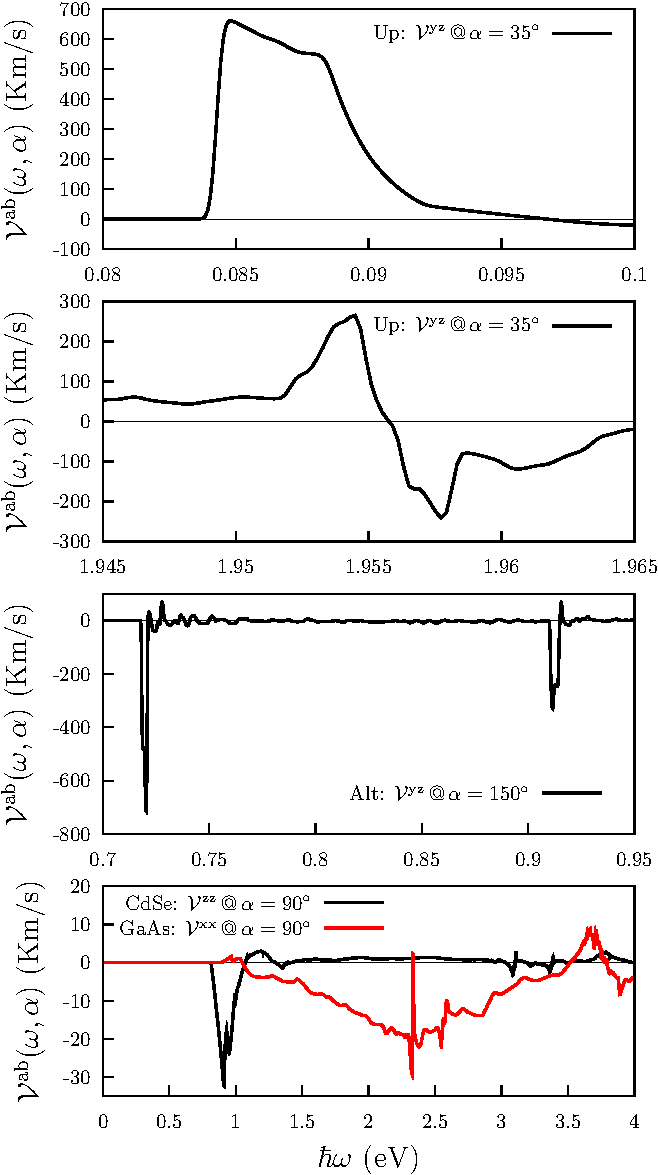
\includegraphics[width=\linewidth]{plots/vab-str-comp}
    
    \caption{Comparison of most intense responses of
    $\mathcal{V}^{\mathrm{ab}}$ for 2D \emph{Alt} and \emph{Up}, and bulk CdSe
    and GaAs structures and their corresponding polarization angle $\alpha$.}
    \label{fig:vab-str-comp}
\end{figure}

Using  Eq. \eqref{eq:vab-aw}, we calculated 
$\mathcal{V}^{\mathrm{ab}}(\omega,\alpha)$ for the \emph{Up} and
\emph{Alt} 2D structures and for CdSe and GaAs which are bulk systems; 
the results
are presented in Fig. \ref{fig:vab-str-comp}. 
The angle $\alpha$ presented in
the response of each structure is that for which the response is maximized in
each case.
% 
The most intense response corresponds to the \emph{Alt} structure centered at
0.720\,eV corresponding to the short-wavelength infrared radiation (SWIR) and
reaching a $\calv^{\rmy\rmz}=-722.2$ Km/s, which means the electrons moving
along $y$ (parallel to the surface) with the spin polarized along $z$
(perpendicular to the surface), with a speed of -722.2 Km/s.
% 
For an energy range from 0.66\,eV to 3.0\,eV, corresponding to energies of the
Near Infrared (NIR) to visible radiation (VIS), the \emph{Up} structure has two
peaks centered at 1.954\,eV and 1.958\,eV reaching $\calv^{\rmy\rmz}=293.9$
Km/s and $\calv^{\rmy\rmz}=-273.0$ Km/s and the \emph{Alt} structure one more
peak centered at 0.0.911\,eV reaching $\calv^{\rmy\rmz}=-357.83$ Km/s.
% 
Then, for the bulk structures we have that the CdSe has only one intense
response centered at 0.912\,eV reaching $\calv^{\rmz\rmz}=-32.3$ Km/s, and the
GaAs structure response reaches the maximum centered at 2.326\,eV reaching
$\calv^{\rmx\rmx}=\calv^{\rmy\rmy}=--28.9$ Km/s.
% 
In table \ref{tab:vab-str-comp} we present the comparison of these values for
the 2D and bulk structures; a positive (negative) spin-velocity means that the
velocity moves (anti-)parallel to the electric field.
% 
We remark that the 2D structures have resonances that give larger values for
$\calv^{\rma\rmb}$ than the bulk crystals; in particular the \emph{Alt}
structure is $\sim 22$ times more intense.



%%%%%%%%%%%%%%%%%%%%%%%%%%%%%%%%%%%%%%%%%%%%%%%%%%%%%%%%%%%%%%%%%%%%%%%%%%%%%%
%%%%%%%%%%%%%%%%%%%%%%%%%%%% Results: Fixing spin %%%%%%%%%%%%%%%%%%%%%%%%%%%%
%%%%%%%%%%%%%%%%%%%%%%%%%%%%%%%%%%%%%%%%%%%%%%%%%%%%%%%%%%%%%%%%%%%%%%%%%%%%%%


\subsection{Fixing spin} % (fold)
\label{sec:res-fixspin}


%%%%%%%%%%%%%%%%%%%%%%%%%%%%%%%%%%%%%%%%%%%%%%%%%%%%%%%%%%%%%%%%%%%%%%%%%%%%%%
%%%%%%%%%%%%%%%%%%%%%%%%%%% Res: fixing spin Up  %%%%%%%%%%%%%%%%%%%%%%%%%%%%%


\begin{figure}[t]
    \centering
    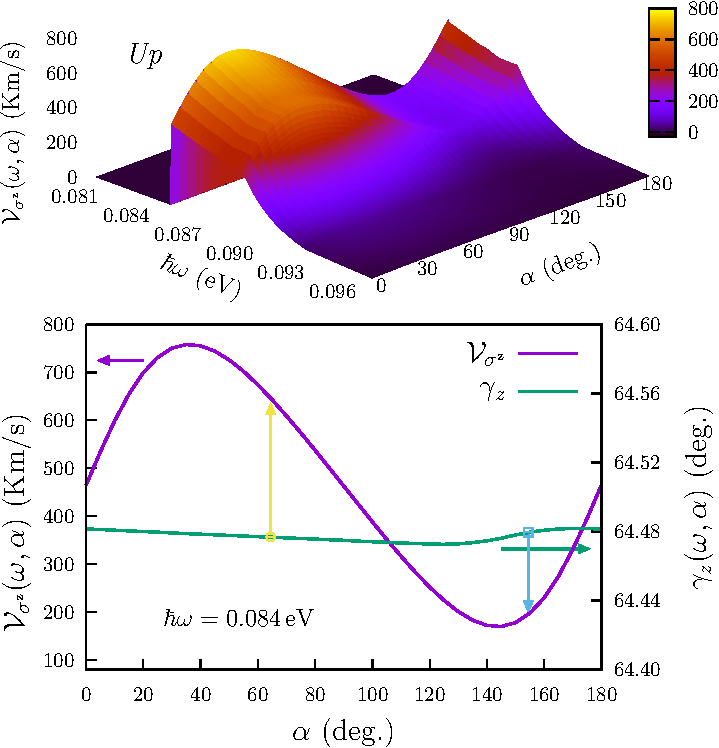
\includegraphics[width=\linewidth]{upplots/up-vsz-w1}
    \caption{Caption here}
    \label{fig:up-vsz-w1}
\end{figure}

\begin{figure}[t]
    \centering
    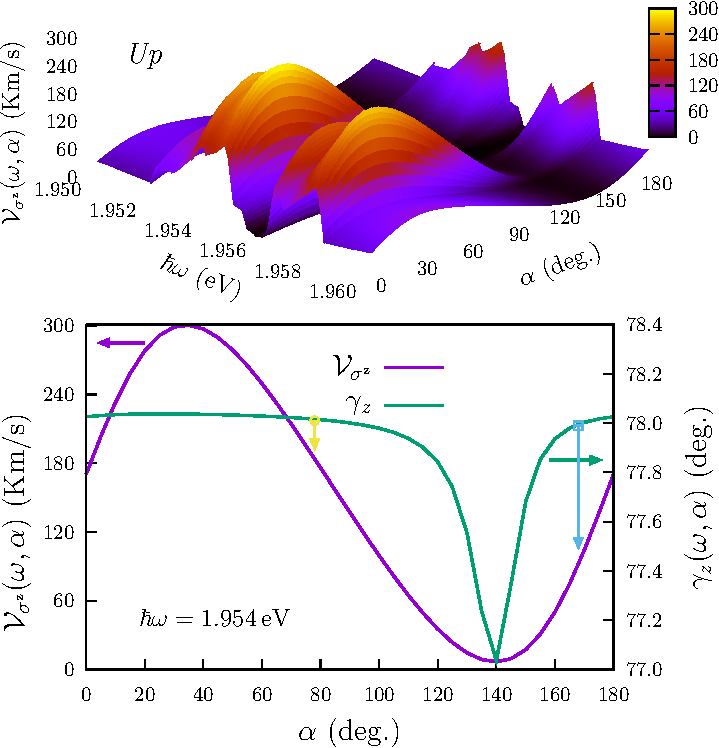
\includegraphics[width=\linewidth]{upplots/up-vsz-w2}
    \caption{caption here}
    \label{fig:up-vsz-w2}
\end{figure}

% %%%%%%%%%%%%%%%%%
% %% 0.0 eV - 0.16 eV  &  1.80 ev - 2.1 ev
% %% Description of UP |V_{s^z}| 3D
% %%%%%%%%%%%%%%%%%

Using Eq. \eqref{eq:vs-mag}, we calculated $\mathcal{V}_{\sigma^{\mathrm{b}}}
(\omega,\alpha)$ and made the analysis for the case when the spin is fixed
along $z$, i.e. directed perpendicularly to the surface of the \emph{Up} and
\emph{Alt} structures. Also, using Eq. \eqref{eq:gamma-ang}, we determined the
angle $\gamma_{\mathrm{b}}(\omega,\alpha)$ where the spin-velocity is directed
along the surface of the each structure.
% 

\subsubsection{\emph{Up} structure}\label{up:fs}

We present in Figs. \ref{fig:up-vsz-w1} and \ref{fig:up-vsz-w2}
$\mathcal{V}_{\sigma^{\mathrm{z}}} (\omega,\alpha)$ for the two energy ranges
of the \emph{Up} structure that give the highest values for $\calv^{\rmy\rmz}$
shown in Fig.~\ref{fig:vab-str-comp}.
% 
We obtain that the zone where the maximum response is reached corresponds to a
energy range of the incident beam from 0.084\,eV to 0.093\,eV, corresponding to
the LWIR, and polarization angles $\alpha$ between $35^{\circ}$ and
$55^{\circ}$. Also,  two local maxima are held for same $\ga$ between
$35^{\circ}$ and $55^{\circ}$, but for an energy range between 1.950\,eV and
1.960\,eV, in the VIS range.
% %%%%%%%%%%%%%%%%% 
% %% 0.0 eV - 0.16 eV
% %% Description of UP |V_{s^z}| & gamma  vs. alpha agle
% %%%%%%%%%%%%%%%%%

In bottom panel of Fig. \ref{fig:up-vsz-w1} we first analyze the response for
$\hbar\go= 0.084$ eV which gives the maximum. We show
$\mathcal{V}_{\sigma^{\mathrm{z}}} (\omega,\alpha)$ as a function of $\ga$
(left scale, black solid line). The absolute maximum is obtained when $\alpha =
35^{\circ}$ resulting in a value of $\mathcal{V}_{\sigma^{\mathrm{z}}}
(\omega,\alpha) = 758.2$\,Km/s, that according to Eq.~\eqref{eq:vs-mag} comes
from $\mathcal{V}^{\mathrm{xz}}(\omega,\alpha) = 326.7$\,Km/s and
$\mathcal{V}^{\mathrm{yz}}(\omega,\alpha) = 684.2$\,Km/s.
% 
In the same panel we present the corresponding velocity angle
$\gamma_{\mathrm{z}}(\omega,\alpha)$ (right scale, red line), that for the
absolute maximum at $\ga = 35^\circ$ is $\gamma_{\mathrm{z}}(\hbar\omega =
0.084\text{eV},\alpha = 35^\circ) = 64.475^{\circ}$. This results means that at
$\hbar\go=0.084$ eV and a polarization angle of the incoming electric field of
$\ga = 35^\circ$ the electrons with a spin pointing along $z$ move at angle of
$\gamma_{\mathrm{z}}(\hbar\omega = 0.084\text{eV},\alpha=35^\circ) \sim
64.5^{\circ}$ with respect to the $x$ direction, with a  maximum speed
$\mathcal{V}_{\sigma^{\mathrm{z}}} (\omega,\alpha)$ of  758.2 Km/s. Also, from
Eq. \eqref{eq:gamma-par} we find that
$\gamma^\parallel_{\mathrm{z}}(\omega,\alpha)=\ga=64.475^\circ$, with
$\mathcal{V}_{\sigma^{\mathrm{z}}}(\omega,\alpha) = 646.0$ Km/s (see green
arrow), and that from Eq. \eqref{eq:gamma-perp},
$\gamma^\perp_{\mathrm{z}}(\omega,\alpha)=\ga-90^\circ=64.47^\circ$, gives
$\ga=154.47^\circ$, with $\mathcal{V}_{\sigma^{\mathrm{z}}}(\omega,\alpha) =
195.6$ Km/s (see blue arrow); thus, for $\hbar\go=0.084$ eV, an $\alpha \sim
65.47^\circ$ ($\alpha \sim 154.5^\circ$) gives electrons with spin polarized
along $z$ moving parallel (perpendicular) to the incident electric field,  with
a speed of 646.0 (195.6) Km/s.
% 
We also find that for all values of $\ga$, $\gamma_{\mathrm{z}}(\omega,\alpha)
\sim 64.48^{\circ}$, being almost constant, and 180.0 Km/s
$<\calv_{\gs^z}(\go,\ga)<$ 758.2 Km/s.

In the bottom panel of Fig. \ref{fig:up-vsz-w2}, now we take
$\hbar\go=1.954$ eV which is the local maximum 
shown in the to panel of same figure. 
The local maximum is
again at  $\alpha = 35^{\circ}$ with
$\mathcal{V}_{\sigma^{\mathrm{z}}} (\omega,\alpha) =
300.4$ Km/s and $\gamma_{\mathrm{z}}(\omega,\alpha) =
78.0^{\circ}$.
% 
In this case, $\alpha =\gamma_{\mathrm{z}}^\parallel(\omega,\alpha) =
78.0^{\circ}$ with $\mathcal{V}_{\sigma^{\mathrm{z}}}(\omega,\alpha) =183.7$
Km/s (green circled box and arrow), and
$\gamma_{\mathrm{z}}^\perp(\omega,\alpha) = 78.0^{\circ}$, for $\alpha =168.0^
{\circ}$ (blue squared box and arrow).
% 
We find  that the velocity angle is almost constant having a range from
$77^{\circ}$ to $78.04^{\circ}$ for  $0^{\circ} \leq
\alpha \leq 180^{\circ}$, and 6.8 Km/s $<\calv_{\gs^z}(\go,\ga)<$ 300.4 Km/s.
% 
Although no figures are presented, we also made the analysis for the
cases when the spin polarization is directed 
along $\mathrm{x}$ and $\mathrm{y}$, finding 
the maxima for
$\hbar\go=0.084$ eV and $\alpha=35^{\circ}$, with
$\mathcal{V}_{\sigma^{\mathrm{x}}}(\omega,\alpha)=219.6$ Km/s and
$\mathcal{V}_{\sigma^{\mathrm{y}}}(\omega,\alpha)=280.3$ Km/s,
$\gamma_{\mathrm{x}}(\omega,\alpha) = 79.3^{\circ}$, and 
$\gamma_{\mathrm{y}}(\omega,\alpha) = 78.2^{\circ}$.

%%%%%%%%%%%%%%%%%%%%%%%%%%%%%%%%%%%%%%%%%%%%%%%%%%%%%%%%%%%%%%%%%%%%%%%%%%%%%%
%%%%%%%%%%%%%%%%%%%%%%%%%%% Res: fixing spin Alt  %%%%%%%%%%%%%%%%%%%%%%%%%%%%

\begin{figure}[tb]
    \centering
    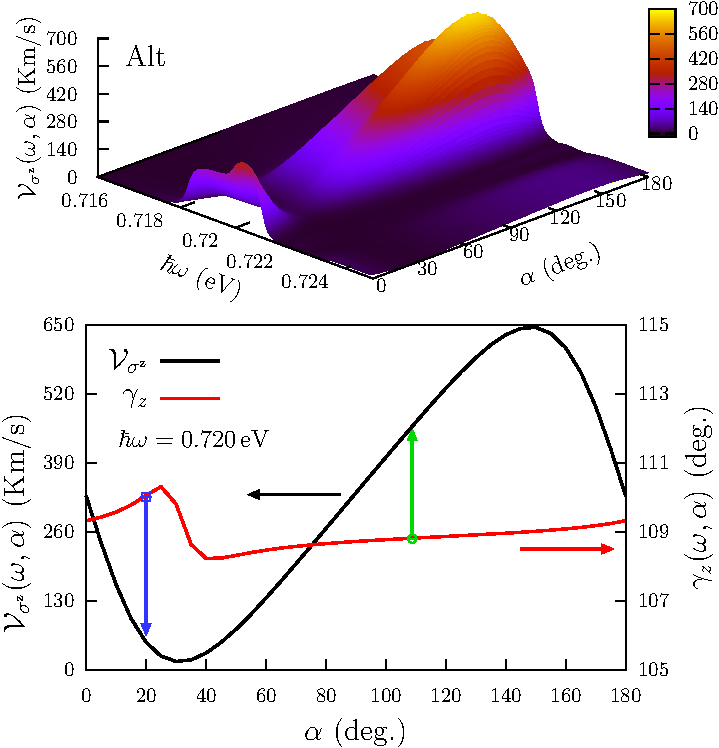
\includegraphics[width=\linewidth]{altplots/alt-vsz}
    \caption{Caption here}
    \label{fig:alt-vsz}
\end{figure}

% %%%%%%%%%%%%%%%%%
% %% 0.0 eV - 0.16 eV  &  1.80 ev - 2.1 ev
% %% Description of ALT |V_{s^z}| 3D
% %%%%%%%%%%%%%%%%%

\subsubsection{\emph{Alt} structure}

We proceed to analyze the $\emph{Alt}$ structure, just as we did the \emph{Up}
structure. Fig. \ref{fig:alt-vsz} shows $\mathcal{V}_{\sigma^{\mathrm{z}}}
(\omega,\alpha)$ (Eq. \eqref{eq:vs-mag}), where we see that the maximum
response is reached for $\hbar\go=0.720$ eV and a local maximum is obtained at
$\hbar\go=0.912$ eV, both located in the short-wavelength infrared radiation
(SWIR) range and for polarization angles, $\ga$,  between $135^{\circ}$ and
$160^{\circ}$.

% %%%%%%%%%%%%%%%%%
% %% 0.0 eV - 0.16 eV
% %% Description of ALT |V_{s^z}| & gamma  vs. alpha agle
% %%%%%%%%%%%%%%%%%
In bottom panel of Fig. \ref{fig:alt-vsz} we plot $\calv_{\gs^z}(\go,\ga)$ vs.
$\ga$ (left scale, black line), fixing the energy to 0.720 eV. The absolute
maximum is obtained for $\alpha = 150^{\circ}$ with
$\mathcal{V}_{\sigma^{\mathrm{z}}} (\omega,\alpha) = 763.5$ Km/s.
% 
In the same panel we present the velocity angle
$\gamma_{\mathrm{z}}(\omega,\alpha)$ vs $\ga$ (right scale, red line), that for
the absolute maximum is $\gamma_{\mathrm{z}}(\omega,\alpha) = 108.9^{\circ}$.
% 
Also, the green circle indicates the value of $\ga$ for which the electrons
move parallel to the incoming electric field, i.e. $\alpha =
\gamma_{\mathrm{z}}^\parallel(\omega,\alpha) = 108.7^{\circ}$, with
$\mathcal{V}_{\sigma^{\mathrm{z}}}(\omega,\alpha) = 511.3$ Km/s. Likewise, the
blue circle indicates the value of $\ga$ for which the electrons move
perpendicular to the incoming electric field, i.e. $\alpha=19.8^{\circ}$, with
$\gamma_{\mathrm{z}\perp}(\omega,\alpha)=109.8^{\circ}$, and
$\mathcal{V}_{\sigma^{\mathrm{z}}} (\omega,\alpha)=61.5$ Km/s.
% 
We also have that $\gamma_{\mathrm{z}}(\omega,\alpha)$ is centered at
$109.1^{\circ}$ having variations of $\pm 0.9^{\circ}$ for $0^{\circ} \leq
\alpha \leq 180^{\circ}$.
% 
Again, for the cases in which the spin polarization is parallel to the surface
the maximum values are $\mathcal{V}_{\sigma^{\mathrm{x}}}(\omega,\alpha) =
297.8$ Km/s and $\mathcal{V}_{\sigma^{\mathrm{y}}}(\omega,\alpha) = 606.4$
Km/s, corresponding to $\gamma_{\mathrm{x}}(\omega,\alpha) = 116.3^{\circ}$
$\gamma_{\mathrm{y}}(\omega,\alpha) = 110.2^{\circ}$ and both for
$\alpha=145^{\circ}$, where the plots are not presented.




%%%%%%%%%%%%%%%%%%%%%%%%%%%%%%%%%%%%%%%%%%%%%%%%%%%%%%%%%%%%%%%%%%%%%%%%%%%%%%
%%%%%%%%%%%%%%%%%%%%%%%%%% Results: Fixing velocity %%%%%%%%%%%%%%%%%%%%%%%%%%
%%%%%%%%%%%%%%%%%%%%%%%%%%%%%%%%%%%%%%%%%%%%%%%%%%%%%%%%%%%%%%%%%%%%%%%%%%%%%%


\subsection{Fixing velocity} % (fold)
\label{sec:res-fixvel}


%%%%%%%%%%%%%%%%%%%%%%%%%%%%%%%%%%%%%%%%%%%%%%%%%%%%%%%%%%%%%%%%%%%%%%%%%%%%%%
%%%%%%%%%%%%%%%%%%%%%%%%%%% Res: fixin vel Up  %%%%%%%%%%%%%%%%%%%%%%%%%%%%%%%

Using the Eq. \eqref{eq:vv-mag}, we calculated the $\mathcal{V}^{\mathrm{a}}
(\omega,\alpha)$ for the cases when the velocity is fixed along the $\rma=x$ or
$\rma=y$ direction on the surface of the \emph{Up} and \emph{Alt} structures,
and from the Eqns. \eqref{eq:polar-ang} and \eqref{eq:azimuthal-ang}, we
determined the polar, $\theta_{\mathrm{a}} (\omega,\alpha)$, and azimuthal,
$\varphi_{\mathrm{a}} (\omega,\alpha)$, angles corresponding to the direction
of the spin.
% 
The plots corresponding to the velocity fixed along the axes as a function of
the energy and polarization angle for the \emph{Up} and \emph{Alt} structures
are similar in shape to the top panels of Figs. \ref{fig:up-vsz-w1}, 
\ref{fig:up-vsz-w2}, and \ref{fig:alt-vsz} and they are not presented here.

\subsubsection{\emph{Up} structure}

% \begin{figure}[t]
%     \centering
%     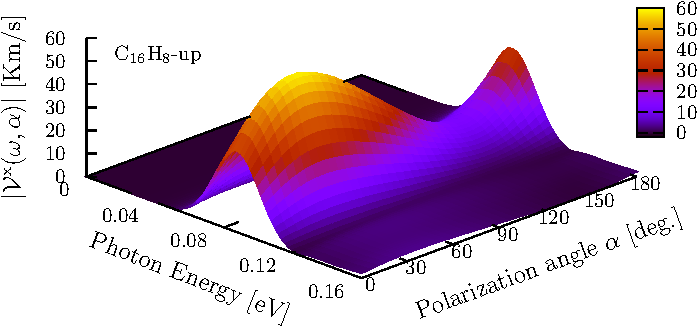
\includegraphics[width=\linewidth]{upplots/up-3d-vxb-1}
%     \\
%     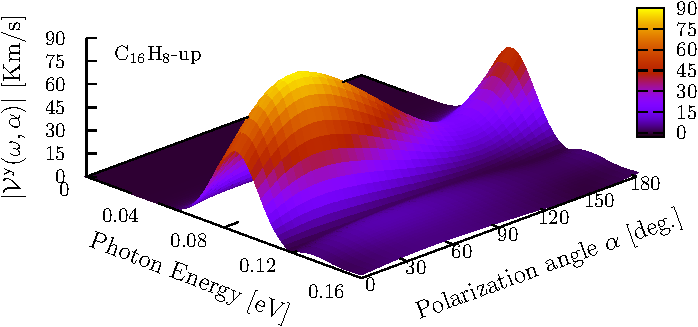
\includegraphics[width=\linewidth]{upplots/up-3d-vyb-1}
%     \caption{ $|\mathcal{V}^{\mathrm{x}}(\omega,\alpha)|$ and
%     $|\mathcal{V}^{\mathrm{y}}(\omega,\alpha)|$responses as a function of the
%     photon energy and polarization angle $\alpha$ for the \emph{Up} structure.
%     The absolute maxima of both are localized in the energy range from 0.08\,eV
%     to 0.10\,eV, in the Far  Infrared, and for polarization angles from
%     $25^{\circ}$ to $50^{\circ}$.}
%     \label{fig:up-3d-vva-1}
% \end{figure}
\begin{figure}[t]
    \centering
    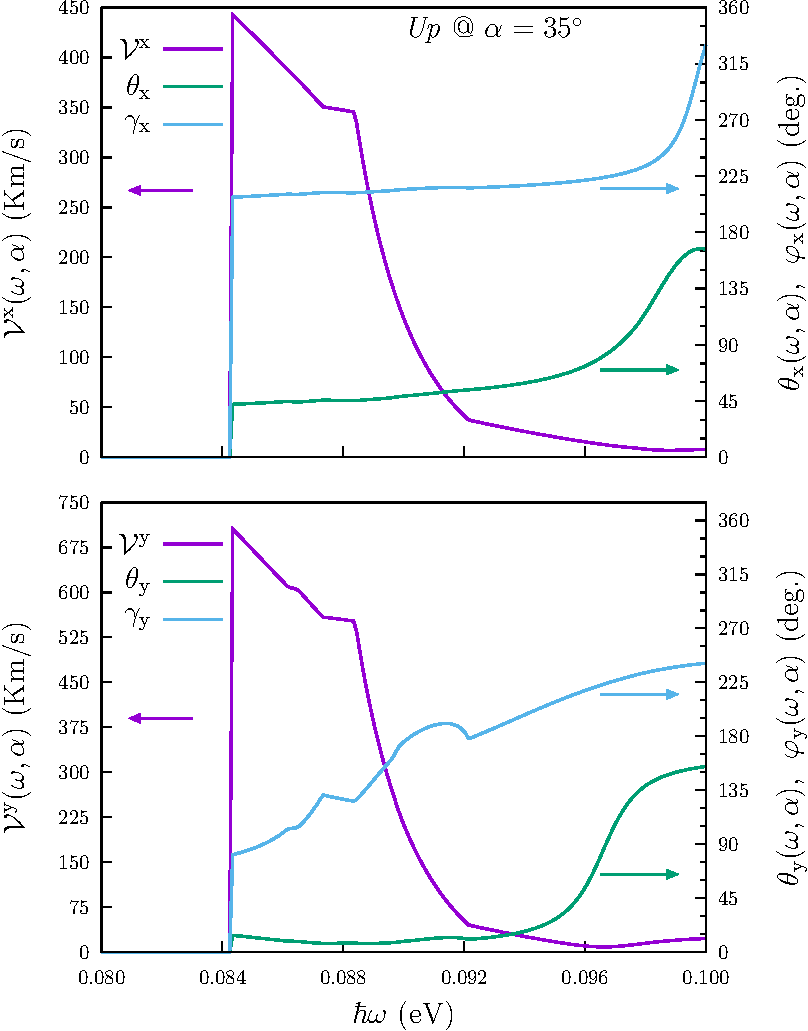
\includegraphics[width=\linewidth]{upplots/up-vx-vy-w1}
    \caption{caption here}
    \label{fig:up-vab-comp-rtp-1}
\end{figure}
% %%%%%%%%%%%%%%%%%
% %% 0.0 eV - 0.16 eV
% %% Description of UP |V^{a}| 3D
% %%%%%%%%%%%%%%%%% 
We proceed to analyze the \emph{Up} structure for the case when the velocity is
directed along the $x$ and $y$ coordinates. We found that each response has a
maximum for $\hbar\omega=0.084$ eV, in the LWIR, and $\ga=35^{\circ}$.
% 
Fixing $\ga=35^{\circ}$, in Fig. \ref{fig:up-vab-comp-rtp-1} we plot
$\mathcal{V}^{\mathrm{x}} (\omega,\alpha)$ and
$\mathcal{V}^{\mathrm{y}}(\omega,\alpha)$ vs. $\hbar\go$ (left scale, black
line) where each responses has a maximum of 442.4\,Km/s and 705.5\,Km/s,
respectively, for $\hbar\go=0.084$ eV.
% 
We also present the corresponding polar (right scale, red line) and azimuthal
(right scale, blue dashed line) spin polarization angles that have values of
% 
$\theta_{\mathrm{x}}(\omega,\alpha) = 42.4^{\circ}$, and
$\varphi_{\mathrm{x}}(\omega,\alpha) = 208.1^{\circ}$ 
% 
when the  electron moves along $x$, and  
$\theta_{\mathrm{y}}(\omega,\alpha) = 14.1^{\circ}$, and
$\varphi_{\mathrm{y}} (\omega,\alpha) = 81.4^{\circ}$, 
% 
when the electron moves along $y$. This means that, the spin is directed upward
the third Cartesian quadrant of the $xy$ plane when the electron moves along
$x$, and is directed almost perpendicularly over the $xy$ plane when it moves
along $y$.
% 
Also, from this figure we have that when the electron moves along $x$ the spin
direction is almost constant for all the energies across the peak of the
response, having a ranges of
% 
$42.4^{\circ} < \theta_{\mathrm{x}}(\omega,\alpha) < 53.6^{\circ} $ 
and $208.1^{\circ} < \varphi_{\mathrm{x}} (\omega,\alpha) < 215.8^{\circ}$. 
% 
Then, when the electron moves along $y$ the spin's polar angle has again
small variations,
% 
$7.6^{\circ} < \theta_{\mathrm{y}} (\omega,\alpha) < 14.1^{\circ}$, 
% 
but in contrast with this the azimuthal angle has significant variations,
% 
$81.4^{\circ} < \varphi_{\mathrm{y}} (\omega,\alpha) < 150.7^{\circ}$.

\begin{figure}[t]
    \centering
    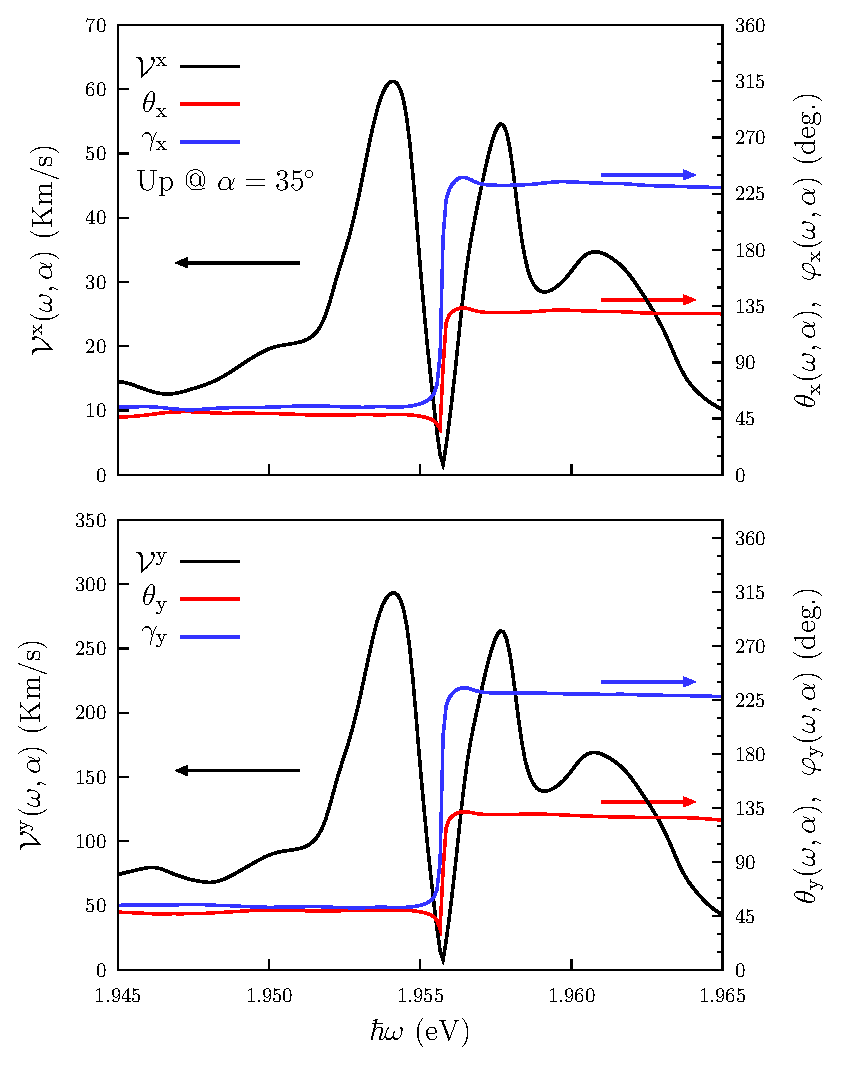
\includegraphics[width=\linewidth]{upplots/up-vx-vy-w2}
    \caption{Caption here}
    \label{fig:up-vx-vy-w2}
\end{figure}
% %%%%%%%%%%%%%%%%%
% %% 1.80 eV - 2.10 eV
% %% Description of UP |V^{a}| 3D
% %%%%%%%%%%%%%%%%%
In  Fig. \ref{fig:up-vx-vy-w2}, for the \emph{Up} structure, we plot
$\mathcal{V}^{\mathrm{a}} (\omega,\alpha)$ vs. $\go$, fixing
$\alpha=35^{\circ}$; the range of $\go$ lies in part of the VIS range. We see
that there are two local maxima at $\hbar\go=1.954$ eV and $\hbar\go=1.958$ eV.
For the first that is the most intense we obtain
% 
$\mathcal{V}^{\mathrm{x}} (\omega,\alpha) =  93.9$ Km/s and  
$\mathcal{V}^{\mathrm{y}} (\omega,\alpha) = 456.3$ Km/s.
% 
For these local maxima, the corresponding polar and azimuthal spin polarization
angles are
% 
$\theta_{\mathrm{x}} (\omega,\alpha) = 48.5^{\circ}$, and 
$\varphi_{\mathrm{x}} (\omega,\alpha) = 54.4^{\circ}$,
% 
for the electron moving along $x$, and
% 
$\theta_{\mathrm{y}} (\omega,\alpha) = 49.9^{\circ}$, and 
$\varphi_{\mathrm{y}} (\omega,\alpha) = 51.8^{\circ}$
% 
for the electron moving along $y$. We remark that these angles are almost
constant for all the energy values across the peak of this local maxima, for
which the spin is directed downward in the third Cartesian quadrant of the $xy$
plane when it moves along either $x$ or $y$ directions. 
% 
For the $\hbar\go=1.958$\,eV peak we obtain 
$\theta_{\mathrm{x}} (\omega,\alpha) = 129.9^{\circ}$, and 
$\varphi_{\mathrm{x}} (\omega,\alpha) = 231.5^{\circ}$, with 
$\mathcal{V}^{\mathrm{x}} (\omega,\alpha) = 88.8$ Km/s, and
% 
$\theta_{\mathrm{y}}(\omega,\alpha) =129.3$, and
$\varphi_{\mathrm{y}}(\omega,\alpha) = 230.4$, with 
$\mathcal{V}^{\mathrm{y}} (\omega,\alpha) = 431.4$ Km/s. 
% 
Again, for this local maxima, the spin angles are almost constant across the
resonant peak.
%%%%%%%%%%%%%%%%%%%%%%%%%%%%%%%%%%%%%%%%%%%%%%%%%%%%%%%%%%%%%%%%%%%%%%%%%%%%%%%
%%%%%%%%%%%%%%%%%%%%%%%%%%% Res: fixin vel Alt  %%%%%%%%%%%%%%%%%%%%%%%%%%%%%%%

\subsubsection{\emph{Alt} structure}

\begin{figure}[tb]
    \centering
    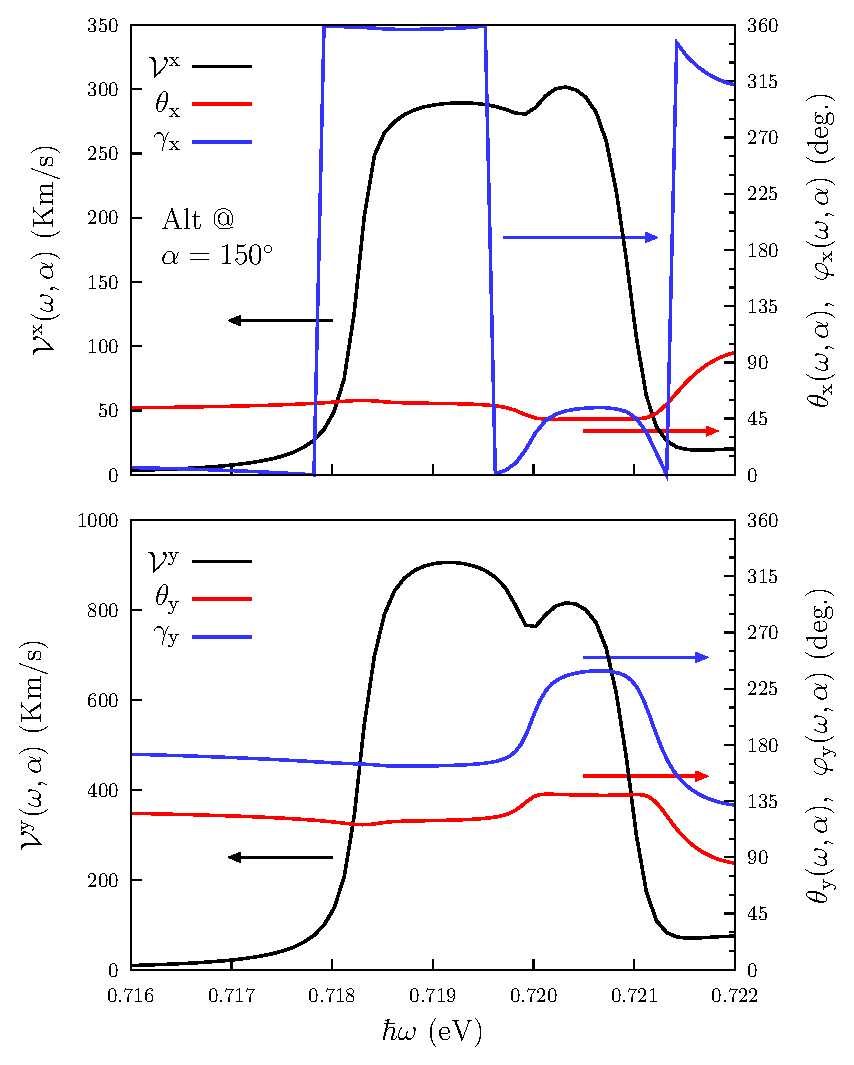
\includegraphics[width=\linewidth]{altplots/alt-vx-vy-w1}
    \caption{Caption here}
    \label{fig:alt-vx-vy-w1}
\end{figure}

\begin{figure}[tb]
    \centering
    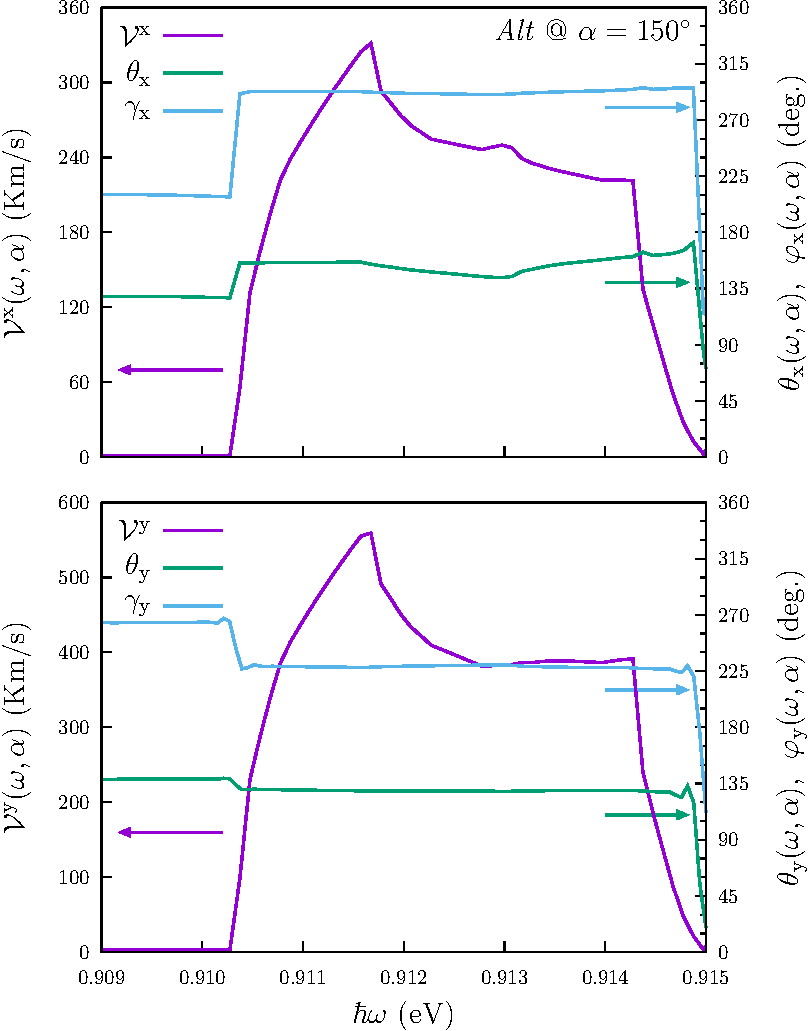
\includegraphics[width=\linewidth]{altplots/alt-vx-vy-w2}
    \caption{Caption here}
    \label{fig:alt-vx-vy-w2}
\end{figure}

In Figs. \ref{fig:alt-vx-vy-w1} and \ref{fig:alt-vx-vy-w2} we show  for the
\emph{Alt} structure $\mathcal{V}^{\mathrm{x}} (\omega,\alpha)$ and
$\mathcal{V}^{\mathrm{y}} (\omega,\alpha)$ as a function of $\omega$, for
$\ga=150^\circ$, the value that maximizes both responses as a function of
$\ga$.
% 
The absolute maxima at $\hbar\go=0.718$ eV gives
% 
$\mathcal{V}^{\mathrm{x}} (\omega,\alpha) =  355.9$ Km/s, and 
$\mathcal{V}^{\mathrm{y}} (\omega,\alpha) = 1008.6$ Km/s, 
% 
and the other one at $\hbar\go=0.911??$ eV gives
% 
$\mathcal{V}^{\mathrm{x}} (\omega,\alpha) = 337.2$ Km/s and
$\mathcal{V}^{\mathrm{y}} (\omega,\alpha) = 568.8$ Km/s.
% 
For $\hbar\go=0.718$ eV,
$\theta_{\mathrm{x}} (\omega,\alpha) = 154.6^{\circ}$, 
$\varphi_{\mathrm{x}}(\omega,\alpha) = 292.2^{\circ}$, 
% 
$\theta_{\mathrm{y}} (\omega,\alpha) = 118.9^{\circ}$, and 
$\varphi_{\mathrm{y}}(\omega,\alpha) = 161.9^{\circ}$, 
% 
implying that the spin is directed over the first Cartesian quadrant of the
$xy$ plane when the spin velocity is directed along $x$, and directed downward
the third Cartesian quadrant when the spin velocity is directed along $y$.
% 
Finally, for $\hbar\go=0.912$ eV, 
% 
$\theta_{\mathrm{x}}(\omega,\alpha) = 153.8^{\circ}$, 
$\varphi_{\mathrm{x}} (\omega,\alpha) = 290.4^{\circ}$,
$\theta_{\mathrm{y}} (\omega,\alpha) = 129.0^{\circ}$, and
$\varphi_{\mathrm{y}} (\omega,\alpha) =228.9^{\circ}$, 
% 
and the spin is directed downward in the fourth Cartesian quadrant of the $xy$
plane when the spin velocity is directed along $x$ and downward the third
Cartesian quadrant when the spin velocity is directed along $y$.

\section{Conclusions} % (fold)
\label{sec:conclusions}

We have performed an \emph{ab initio} calculation for the SVI by one-photon
absorption of linearly polarized light in the \emph{Up} and \emph{Alt} 2D
hydrogenated graphene structures that and we made the calculation for the case
when the spin is polarized in the $z$ direction or when the velocity is
directed along $x$ or $y$; this effect does not seem to have been reported
previously. 
% 
This SVI is very sensitive to the symmetry characteristics of the structures
presenting an anisotropic behavior. We found that the \emph{Up} structure has
the most intense response for the spin directed along $z$ resulting in 
% 
$\mathcal{V}_{\sigma^{\mathrm{z}}} (\omega,\alpha) = 758.2$\,Km/s and 
% 
for an energy of the incoming beam of 0.084\,eV. Also the \emph{Alt} structure
has the most intense response when the spin moves along the $y$ direction
resulting in 
% 
$\mathcal{V}^{\mathrm{y}} (\omega,\alpha) = 1008.6$\,Km/s
% 
for an energy of the incoming beam of 0.718\,eV.
% 
The spin relaxation time in pure and doped graphene is long enough in the order
from nanoseconds to milliseconds. \cite{wojtaszekPRB13,ertlerPRB09} The,
according to our results both are excellent candidates for the development of
spintronics devices that require PSC due to the high spin velocity transport.

\section{Acknowledgment} % (fold)

This work has been supported by \emph{Consejo Nacional de Ciencia y
Tecnolog\'ia} (CONACyT), M\'exico, Grant No. 153930.

\bibliography{article.bib}

\end{document}
